\documentclass[11pt]{report}
\usepackage{blindtext}
\usepackage[margin=1in]{geometry}
\usepackage{graphicx}
\usepackage{verbatim}
\title{Thanks Corporation Database Project\\CMSI 486 Enterprise Project\\Fall 2014}
\author{Edward Bramanti}
\date{This project designs and implements a database for an employee recognition system for companies to use internally.}

\providecommand\phantomsection{}


\renewcommand\thechapter{\Roman{chapter}}
\renewcommand\thesection{\thechapter.\arabic{section}}

\usepackage{tocloft}
\setlength{\cftchapnumwidth}{3em}
\setlength{\cftsecnumwidth}{3.5em}
\setlength{\cftsubsecnumwidth}{4em}

\begin{document}
\clearpage
\phantomsection
\addcontentsline{toc}{chapter}{
    \protect\numberline{I}Title Page}
\maketitle
\clearpage
\phantomsection
\addcontentsline{toc}{chapter}{
    \protect\numberline{II}Table of Contents}
\tableofcontents
\setcounter{page}{2}
\setcounter{chapter}{2}
\chapter{Description of the Enterprise}

Thanks is an effective, entirely digital, multi-purpose employee recognition system. The database will consist of many different companies who will pay for a service that makes recognizing employees simple and meaningful. This will allow the Thanks database to be used in a way that is unique to each company using the service.

The enterprise in question will make it much easier for employees to recognize one another across their company. As companies grow, it becomes difficult to maintain an atmosphere of employee worth. This growing size represents a problem as individual employees can feel like their work goes unnoticed in their company. “Thanks” provides a remedy for that by providing a digital way to send recognition to any employee quickly.

In an organization, there will be one user type with some special attributes. For example, an executive will be a special user type and will be denoted with special attributes. When opening the thanks form, it will be necessary to present a list of all employees in the company. A list of employees would appear with these attributes: name, position and department. This would provide employees with a clear snapshot on everyone’s role in the company if they saw a fellow employee do something amazing and was not sure what position they occupied in the company. Users will be able to send other users the primary data type known as Thanks. For each thank, we have a user that gives the Thanks and a user that receives the Thanks. This demonstrates the personal aspect of recognition, as an employee recognizes a specific employee directly.

A Thanks also contains an area for an employee to write a message so they can explain what they are thanking the employee for. This allows for personalization of the Thanks so that employees can be detailed on the outstanding work their coworkers are doing. Finally, companies will be able to define a custom attribute for the last part of the Thanks, which will be represented as values the company wants to promote. The advantage of this value is that companies, depending on their mission statements and core beliefs, will be able to tailor this field to encourage specific attributes that represent the company within employees.

Thanks represents a social network within a company than it is a private thanking system. Messages will display on a live feed all of the “Thanks” being given around the company. Employees will be able to easily see the interaction and encouragement being spread amongst their acquaintances. The potential of “Thanks” is enormous, which is why a specific structure around a public space of thanks combined with personalized instances and explanations of employee worth are necessary in this database design.\\

\clearpage
Here are a set of questions employees, department heads or executives may pose when retrieving data:
\begin{enumerate}
    \item List the names of all employees in the company.
    \item Which department has received the most Thanks in the company?
    \item Return a list of all employees who have nicknames.
    \item List all company values for the company.
    \item Which department head has received the most Thanks in the company?
    \item Which one of an employee's thanks they gave received the most likes?
    \item Who has never received a Thanks within a company?
    \item Who is the newest employee to have joined the company?
    \item What Thanks were posted in the database on October 20, 2014?
    \item List the executives in the company.
\end{enumerate}

\chapter{Definition of Environment}

\section{Input and Report Forms}
\begin{itemize}
    \item Thanks Form
    \begin{itemize}
        \item Name of Employee Being Thanked
        \item Message
        \item Company Value (optional) \\
        Represents a custom value that the company wants to encourage in their employees
    \end{itemize}
    \item Employee Profile Page \\
    Allows for editing of a specific employee's profile. Some of the values stored in the database will not be able to be changed, such as Real Name and Job Title, and must be updated by an admin.
    \begin{itemize}
        \item Edit Employee's Nickname
        \item Edit Employee's Photo
    \end{itemize}
    \item ``Thanks Feed'' of Company \\
    Allows employees to see the ``Thanks Feed'' of the company, a place where signed-in employees can like Thanks messages that have been given and comment/like those thanks messages.
    \item Thanks Item in ``Thanks Feed'' \\
    Allows an employee to take action on a Thanks item within the ``Thanks Feed''.
    \begin{itemize}
        \item Like Current Message \\
        Allows employee to like a Thanks Given, whether it's directly to/from or external from the employee.
        \item Comment on Current Message \\
        A comment is a text response to a Thanks Given, whether it's directly to/from or external from the employee.
    \end{itemize}
    \item Admin Panel for Department \\
    Allows for department heads to manage information about their department.
    \begin{itemize}
        \item Edit Department Title \\
        If the title of a department changes slightly, a department head is able to change this.
        \item Edit Department Description \\
        Allows department head to change the department description information.
        \item Edit Department Employee's Job Title \\
        Allows department head to select a specific employee's job title in their department and edit it.
    \end{itemize}
    \item Admin Panel for Executive \\
    Allows for executives to manage information about their company, and to change even department-level information.
    \begin{itemize}
        \item Edit Company Title \\
        Allows executives to change their company name if their corporation undergoes a name change.
        \item Edit Company Founded Date \\
        Allows executives to set the founding date of the company.
        \item Set Department Heads \\
        Allows executives to set the head of each department.
    \end{itemize}
    \item Webmaster Panel for DB Manager \\
    Since Thanks Corporation is a business that provides its database service to other companies, a webmaster needs an admin panel to manage the many companies in the database.
    \begin{itemize}
        \item View Companies in Database \\
        Allows webmaster to view all companies in the database
        \item Edit Companies in Database \\
        Allows webmaster to deactivate companies or remove companies from database.
    \end{itemize}
\end{itemize}
\clearpage
\section{Assumptions}
\begin{enumerate}
\item Fellow employees address thanks to other employees.
\item Each employee gets their own account, which has predefined data and some limited customization/personalization.
\item Employees can view a newsfeed-like interface of all thanks being given throughout the company.
\item Employees have the ability to like and comment on all Thanks company-wide.
\item Department heads will be able to manage their department info and certain employee info.
\item Executives will be able to manage department heads and company info.
\end{enumerate}
\clearpage
\section{User-Oriented Data Dictionary}
\begin{table}[h]
\begin{tabular}{|l|l|}
\hline
\multicolumn{1}{|c|}{\textbf{Datum}} & \multicolumn{1}{c|}{\textbf{Information Definition}}                            \\ \hline
comment\_data                        & Text data contained within a comment on a Thanks data type                      \\ \hline
companies                            & View of companies for a webmaster of Thanks                                     \\ \hline
company\_title                       & Title of a company using Thanks                                                 \\ \hline
company\_value                       & Value being exuding that represents the company in the Thanks \\ \hline
department\_description              & Description of particular department in text form                               \\ \hline
department\_title                    & The name of a particular department within the company                          \\ \hline
employee\_department                 & Department employee works in                                                    \\ \hline
employee\_name                       & Name of employee in the company, form                                           \\ \hline
employee\_nickname                   & Nickname of an employee                                                         \\ \hline
employee\_photo                      & Photo of an employee for the Thanks database                                    \\ \hline
employee\_title                      & Job title of an employee’s position                                             \\ \hline
founded\_date                        & Date that a company was founded                                                 \\ \hline
like\_data                           & Stored when an employee likes a Thanks another employee game                    \\ \hline
message\_data                        & Text data contained within the body of a Thanks data type                       \\ \hline
thanks\_feed                         & List of all Thanks in a corporation                                             \\ \hline
\end{tabular}
\end{table}
\clearpage
\section{Cross-Reference Table}
\begin{table}[h]
\centering
\resizebox{\textwidth}{!}{%
\begin{tabular}{|l|c|cccccc}
\cline{1-2}
\multicolumn{1}{|c|}{\textbf{Datum}} & \textbf{Form/Screen} &                                       &                                    &                                  &                                             &                                            &                                            \\ \hline
\multicolumn{1}{|c|}{\textbf{}}      & \textbf{Thanks Form} & \multicolumn{1}{c|}{\textbf{Employee Profile}} & \multicolumn{1}{c|}{\textbf{"Thanks Feed"}} & \multicolumn{1}{c|}{\textbf{Thanks Item}} & \multicolumn{1}{c|}{\textbf{Department Admin Panel}} & \multicolumn{1}{c|}{\textbf{Executive Admin Panel}} & \multicolumn{1}{c|}{\textbf{Webmaster Admin Panel}} \\ \hline
comment\_data                        &             & \multicolumn{1}{c|}{}                 & \multicolumn{1}{c|}{X}             & \multicolumn{1}{c|}{X}           & \multicolumn{1}{c|}{}                       & \multicolumn{1}{c|}{}                      & \multicolumn{1}{c|}{}                      \\ \hline
companies                            &             & \multicolumn{1}{c|}{}                 & \multicolumn{1}{c|}{}              & \multicolumn{1}{c|}{}            & \multicolumn{1}{c|}{}                       & \multicolumn{1}{c|}{}                      & \multicolumn{1}{c|}{X}                     \\ \hline
company\_title                       &             & \multicolumn{1}{c|}{}                 & \multicolumn{1}{c|}{X}             & \multicolumn{1}{c|}{}            & \multicolumn{1}{c|}{}                       & \multicolumn{1}{c|}{X}                     & \multicolumn{1}{c|}{}                      \\ \hline
company\_value                       & X           & \multicolumn{1}{c|}{}                 & \multicolumn{1}{c|}{}              & \multicolumn{1}{c|}{}            & \multicolumn{1}{c|}{}                       & \multicolumn{1}{c|}{}                      & \multicolumn{1}{c|}{}                      \\ \hline
department\_description              &             & \multicolumn{1}{c|}{}                 & \multicolumn{1}{c|}{}              & \multicolumn{1}{c|}{}            & \multicolumn{1}{c|}{X}                      & \multicolumn{1}{c|}{}                      & \multicolumn{1}{c|}{}                      \\ \hline
department\_title                    &             & \multicolumn{1}{c|}{}                 & \multicolumn{1}{c|}{}              & \multicolumn{1}{c|}{}            & \multicolumn{1}{c|}{X}                      & \multicolumn{1}{c|}{}                      & \multicolumn{1}{c|}{}                      \\ \hline
employee\_department                 &             & \multicolumn{1}{c|}{X}                & \multicolumn{1}{c|}{}              & \multicolumn{1}{c|}{X}           & \multicolumn{1}{c|}{}                       & \multicolumn{1}{c|}{}                      & \multicolumn{1}{c|}{}                      \\ \hline
employee\_name                       & X           & \multicolumn{1}{c|}{X}                & \multicolumn{1}{c|}{}              & \multicolumn{1}{c|}{X}           & \multicolumn{1}{c|}{X}                      & \multicolumn{1}{c|}{X}                     & \multicolumn{1}{c|}{}                      \\ \hline
employee\_nickname                   &             & \multicolumn{1}{c|}{X}                & \multicolumn{1}{c|}{}              & \multicolumn{1}{c|}{X}           & \multicolumn{1}{c|}{X}                      & \multicolumn{1}{c|}{X}                     & \multicolumn{1}{c|}{}                      \\ \hline
employee\_photo                      &             & \multicolumn{1}{c|}{X}                & \multicolumn{1}{c|}{}              & \multicolumn{1}{c|}{X}           & \multicolumn{1}{c|}{}                       & \multicolumn{1}{c|}{}                      & \multicolumn{1}{c|}{}                      \\ \hline
employee\_title                      &             & \multicolumn{1}{c|}{X}                & \multicolumn{1}{c|}{}              & \multicolumn{1}{c|}{X}           & \multicolumn{1}{c|}{X}                      & \multicolumn{1}{c|}{X}                     & \multicolumn{1}{c|}{}                      \\ \hline
founded\_date                        &             & \multicolumn{1}{c|}{}                 & \multicolumn{1}{c|}{}              & \multicolumn{1}{c|}{}            & \multicolumn{1}{c|}{}                       & \multicolumn{1}{c|}{X}                     & \multicolumn{1}{c|}{}                      \\ \hline
like\_data                           &             & \multicolumn{1}{c|}{}                 & \multicolumn{1}{c|}{X}             & \multicolumn{1}{c|}{X}           & \multicolumn{1}{c|}{}                       & \multicolumn{1}{c|}{}                      & \multicolumn{1}{c|}{}                      \\ \hline
message\_data                        & X           & \multicolumn{1}{c|}{}                 & \multicolumn{1}{c|}{X}             & \multicolumn{1}{c|}{X}           & \multicolumn{1}{c|}{}                       & \multicolumn{1}{c|}{}                      & \multicolumn{1}{c|}{}                      \\ \hline
thanks\_feed                         &             & \multicolumn{1}{c|}{}                 & \multicolumn{1}{c|}{X}             & \multicolumn{1}{c|}{}            & \multicolumn{1}{c|}{}                       & \multicolumn{1}{c|}{}                      & \multicolumn{1}{c|}{}                      \\ \hline
\end{tabular}
}
\end{table}
\clearpage

\chapter{Enterprise Database Design}

\section{Logical Model of the Enterprise}
\subsection{List of Entities and Attributes}

\begin{itemize}
\item Employee
    \begin{itemize}
    \item eid: Employee ID
    \item name: Employee Name
    \item job\_title: Employee Job Title
    \item photo: Employee Photo
    \item nickname: Employee Nickname
    \item started: Date the Employee Started
    \end{itemize}
\item Department Head - inherits Employee
    \begin{itemize}
    \item headid: Department Head ID
    \end{itemize}
\item Executive - inherits Employee
    \begin{itemize}
    \item execid: Executive ID
    \end{itemize}
\item Department
    \begin{itemize}
    \item did: Department ID
    \item depTitle: Department Title
    \item depDescription: Department Description
    \end{itemize}
\item Company
    \begin{itemize}
    \item cid: Company ID
    \item cTitle: Company Title
    \item founded\_date: Date Company was Founded
    \end{itemize}
\item Thanks
    \begin{itemize}
    \item tid: Thanks ID
    \item thanksdate: Date Thanks was Given
    \end{itemize}
\item Like
    \begin{itemize}
    \item likedate: Date Like was Given
    \end{itemize}
\item Comment
    \begin{itemize}
    \item commentdate: Date Comment was Given
    \end{itemize}
\item Message
    \begin{itemize}
    \item mid: Message ID
    \item message\_text: Text of Message
    \end{itemize}
\item Company Value
    \begin{itemize}
    \item vid: Company Value ID
    \item value\_type: type of company value
    \end{itemize}
\end{itemize}
\clearpage

\subsection{List of Relationships and Attributes}
\begin{itemize}
\item Relationship
\end{itemize}
\clearpage

\subsection{Entity-Relationship Diagram of the Enterprise}

\begin{figure}[!htb]
\centering
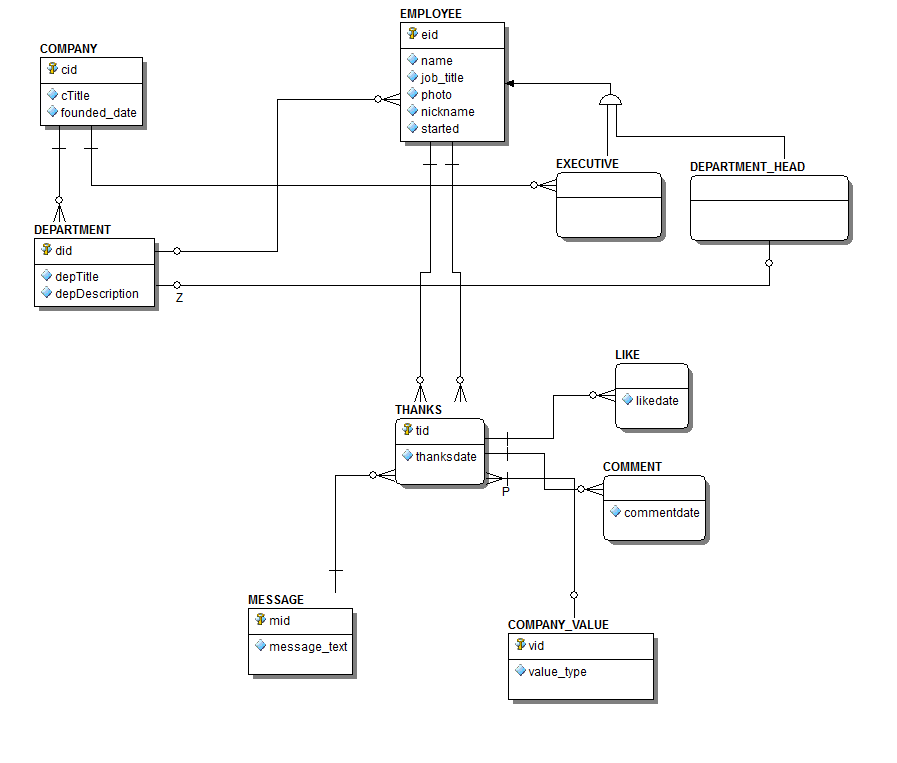
\includegraphics[scale=.7]{./images/ERD11-4.png}
\end{figure}
\clearpage

\section{Conceptual Model of the Enterprise}
A conceptual model of the Thanks database. \\

employee(\underline{eid}, name, job\_title, photo, nickname, started) \\
PK - eid \\
CK - eid, name, photo \\
AK - name, photo \\
FK - employee.did REFERENCES department.did \\

departmenthead(\underline{headid}) \\
PK - headid \\
CK - headid \\

executive(\underline{execid}) \\
PK - execid \\
CK - execid \\
FK - executive.cid REF company.cid \\

department(\underline{did}, depTitle, depDescription) \\
PK - did \\
CK - did \\
FK - department.headid REFERENCES departmenthead.headid \\
     department.cid REFERENCES company.cid \\

company(\underline{cid}, cTitle, founded\_date) \\
PK - cid \\
CK - cid, cTitle \\
AK - cTitle \\

thanks(\underline{(tid, mid)}, thanksdate) \\
PK - (tid, mid) \\
CK - tid \\
FK - thanks.mid REFERENCES message.mid \\
     thanks.to REFERENCES employee.eid \\
     thanks.from REFERENCES employee.eid \\
     thanks.vid REFERENCES company\_value.vid \\

like(\underline{(likeid, mid)}, likedate) \\
PK - (likeid, mid) \\
CK - likeid \\
FK - like.mid REFERENCES message.mid \\

comment(\underline{(commentid, mid)}, commentdate) \\
PK - (commentid, mid) \\
CK - commentid \\
FK - comment.mid REFERENCES message.mid \\

message(\underline{mid}, message\_text) \\
PK - mid \\
CK - mid \\

company\_value(\underline{vid}, value\_type) \\
PK - vid \\
CK - vid \\
\clearpage
\section{Table Dictionary}
\begin{table}[h]
\centering
\resizebox{\textwidth}{!}{%
\begin{tabular}{|l|l|l|}
\hline
\multicolumn{1}{|c|}{\textbf{Table}} & \multicolumn{1}{c|}{\textbf{Attributes}}                & \multicolumn{1}{c|}{\textbf{Definition}}               \\ \hline
EMPLOYEE                             & \underline{eid}, name, job\_title, photo, nickname, started, did    & Employee in a company                                  \\ \hline
DEPARTMENT\_HEAD                     & headid, name, job\_title, photo, nickname, started      & The manager/head of a department                       \\ \hline
EXECUTIVE                            & execid, name, job\_title, photo, nickname, started, cid & Executive in a company                                 \\ \hline
DEPARTMENT                           & did, depTitle, depDescription, headid, cid              & Department in a company                                \\ \hline
COMPANY                              & cid, cTitle, founded\_date                              & Represents a company, which is the starting data point \\ \hline
THANKS                               & tid, thanksdate                                         & Data type used to recognize another employee           \\ \hline
LIKE                                 & likeid, mid, likedate                                   & A like on a Thanks post                                \\ \hline
COMMENT                              & commentid, mid, commentdate                             & A comment on a Thanks post                             \\ \hline
MESSAGE                              & mid, message\_text                                      & Message of a Thanks                                    \\ \hline
COMPANY\_VALUE                       & vid, value\_type                                        & Company value of a Thanks                              \\ \hline
\end{tabular}
}
\end{table}
\clearpage
\section{Attribute Dictionary}
\begin{table}[h]
\centering
\resizebox{\textwidth}{!}{%
\begin{tabular}{|l|l|}
\hline
\multicolumn{1}{|c|}{\textbf{Attribute}} & \multicolumn{1}{c|}{\textbf{Tables Used In}} \\ \hline
eid                                      & EMPLOYEE                                     \\ \hline
headid                                   & DEPARTMENT\_HEAD                             \\ \hline
execid                                   & EXECUTIVE                                    \\ \hline
name                                     & EMPLOYEE, DEPARTMENT\_HEAD, EXECUTIVE        \\ \hline
job\_title                               & EMPLOYEE, DEPARTMENT\_HEAD, EXECUTIVE        \\ \hline
photo                                    & EMPLOYEE, DEPARTMENT\_HEAD, EXECUTIVE        \\ \hline
nickname                                 & EMPLOYEE, DEPARTMENT\_HEAD, EXECUTIVE        \\ \hline
started                                  & EMPLOYEE, DEPARTMENT\_HEAD, EXECUTIVE        \\ \hline
did                                      & DEPARTMENT                                   \\ \hline
depTitle                                 & DEPARTMENT                                   \\ \hline
depDescription                           & DEPARTMENT                                   \\ \hline
cid                                      & COMPANY                                      \\ \hline
cTitle                                   & COMPANY                                      \\ \hline
founded\_date                            & COMPANY                                      \\ \hline
tid                                      & THANKS                                       \\ \hline
thanksdate                               & THANKS                                       \\ \hline
likeid                                   & LIKE                                         \\ \hline
likedate                                 & LIKE                                         \\ \hline
commentid                                & COMMENT                                      \\ \hline
commentdate                              & COMMENT                                      \\ \hline
mid                                      & MESSAGE                                      \\ \hline
message\_text                            & MESSAGE                                      \\ \hline
vid                                      & COMPANY\_VALUE                               \\ \hline
value\_type                              & COMPANY\_VALUE                               \\ \hline
\end{tabular}
}
\end{table}
\clearpage

\chapter{Database and Query Definition}

\section{Database Definition}
\verbatiminput{sql/ThanksCorporation.sql}
\section{Database Queries}
Given below are 11 example English queries, with their SQL DML used to retrieve the necessary data.
\begin{enumerate}
    \item List the names of all employees in the company ``I Love Thanks".
    \begin{verbatim}
    SELECT e.name
    FROM company as c
    INNER JOIN department as d
    ON c.cid = d.cid
    INNER JOIN employee as e
    ON d.did = e.did
    WHERE c.cTitle = "I Love Thanks"
    ;
    \end{verbatim}
    \item Show all department names in the corporation ``Blitz''.
    \begin{verbatim}
    SELECT d.depTitle
    FROM company AS c
    INNER JOIN department as d
    ON c.cid = d.cid
    WHERE c.cTitle = "Blitz"
    ;
    \end{verbatim}
    \item Return a list of all employees in the database who have nicknames.
    \begin{verbatim}
    SELECT e.name, e.nickname
    FROM employee AS e
    WHERE EXISTS (
        SELECT e.nickname
        FROM employee
    )
    ;
    \end{verbatim}
    \item Show names of employees who do not have photos in the ``I Love Thanks" company.
    \begin{verbatim}
    SELECT e.name
    FROM company as c
    INNER JOIN department as d
    ON c.cid = d.cid
    INNER JOIN employee as e
    ON d.did = e.did
    WHERE c.photo IS NULL
    AND c.cTitle = "I Love Thanks"
    ;
    \end{verbatim}
    \item Show all department heads in ``Insomniac Corporation''.
    \begin{verbatim}
    SELECT dh
    FROM company as c
    INNER JOIN department as d
    ON c.cid = d.cid
    INNER JOIN department_head as dh
    ON d.headid = dh.headid
    WHERE c.cTitle = "Insomniac Corporation"
    ;
    \end{verbatim}
    \item Show all of the Thanks that Julia Crow from ``Playa Medical'' gave.
    \begin{verbatim}
    SELECT t
    FROM company as c
    INNER JOIN department as d
    ON c.cid = d.cid
    INNER JOIN employee as e
    ON d.did = e.did
    INNER JOIN thanks as t
    ON t.from = e.eid
    WHERE c.cTitle = "Playa Medical"
    AND e.name = "Julia Crow"
    ;
    \end{verbatim}
    \item Show all of the Thanks that Emma Cross from ``Boeing'' received.
    \begin{verbatim}
    SELECT t
    FROM company as c
    INNER JOIN department as d
    ON c.cid = d.cid
    INNER JOIN employee as e
    ON d.did = e.did
    INNER JOIN thanks as t
    ON t.from = e.eid
    WHERE c.cTitle = "Boeing"
    AND e.name = "Julia Crow"
    ;
    \end{verbatim}
    \item Show all thanks that have been given in the corporation ``First America''.
    \begin{verbatim}
    SELECT t
    FROM company as c
    INNER JOIN department as d
    ON c.cid = d.cid
    INNER JOIN employee as e
    ON d.did = e.did
    INNER JOIN thanks as t
    ON t.to = e.eid
    WHERE c.cTitle = "First America"
    ;
    \end{verbatim}
    \item Who is the newest employee to have joined the company ``Lightning Corporation''?
    \begin{verbatim}
    SELECT e.name
    FROM company as c
    INNER JOIN department as d
    ON c.cid = d.cid
    INNER JOIN employee as e
    ON d.did = e.did
    WHERE c.cTitle = "Lightning Corporation"
    AND e.started = (
        SELECT MAX(e.started)
        FROM company as c
        INNER JOIN department as d
        ON c.cid = d.cid
        INNER JOIN employee as e
        ON d.did = e.eid
        WHERE c.cTitle = "Lightning Corporation"
    )
    ;
    \end{verbatim}
    \item List all thanks posted in the database in October.
    \begin{verbatim}
    SELECT t
    FROM thanks as t
    WHERE MONTHNAME(t.thanksdate) = "October"
    ;
    \end{verbatim}
    \item List the executives in the company ``I Love Thanks".
    \begin{verbatim}
    SELECT e
    FROM company as c
    INNER JOIN executive as e
    ON c.cid = e.cid
    WHERE c.cTitle = "I Love Thanks"
    ;
    \end{verbatim}
\end{enumerate}
\clearpage
\section{Design Tradeoffs and Limitations}

One design tradeoff in its current state is the lack of Thanks being tied to the company. In order to gain access to all thanks by company, multiple joins must be performed instead of having a relationship directly between company and the thanks given within a company. This may be remedied in the future by adding a relationship between THANKS and COMPANY.\\

Another design tradeoff is the lack of relationship between COMPANY and COMPANY\_VALUE. This issue is very similar to the tradeoff listed above: multiple joins are required in order to get the COMPANY\_VALUE when a relationship could be tied between COMPANY and COMPANY\_VALUE.\\

Finally, one design difficulty was in how employees are linked to thanks. Two foreign keys are required in a Thanks entity, which have been aliased to `to' and `from'. Both of these reference an employee, and can create difficulty due to the aliasing of the foreign keys. However, this is necessary in the current implementation.

\end{document}
